\documentclass[conference]{IEEEtran}
\usepackage{cite}
\usepackage{amsmath,amssymb,amsfonts}
\usepackage{algorithmic}
\usepackage{graphicx}
\usepackage{textcomp}
\usepackage[english]{babel}
\usepackage{blindtext}
\usepackage{array}
\def\BibTeX{{\rm B\kern-.05em{\sc i\kern-.025em b}\kern-.08em
    T\kern-.1667em\lower.7ex\hbox{E}\kern-.125emX}}
\begin{document}

\title{Comparison between Genetic Algorithms and Ant Colony Optimization for Multi-Agent Path Planning in 3D}

\author{
\IEEEauthorblockN{Cheng Dong}
\IEEEauthorblockA{\textit{c9dong@edu.uwaterloo.ca}}
\and
\IEEEauthorblockN{Zhaotian Fang}
\IEEEauthorblockA{\textit{z23fang@edu.uwaterloo.ca}}
\and
\IEEEauthorblockN{Zu Qi Li}
\IEEEauthorblockA{\textit{zq6li@edu.uwaterloo.ca}}
\and
\IEEEauthorblockN{Di Sen Lu}
\IEEEauthorblockA{\textit{dslu@uwaterloo.ca}}
\and
\IEEEauthorblockN{YuYang Si}
\IEEEauthorblockA{\textit{y6si@uwaterloo.ca}}
\and
\IEEEauthorblockN{Andrew Zhou}
\IEEEauthorblockA{\textit{a25zhou@edu.uwaterloo.ca}}
}

\maketitle

\begin{abstract}
% TODO: Zuqi
This paper describes the problem of three dimensional path planning for multiple agents, reviews previous research on the subject, and details the application of two meta heuristic algorithms, genetic algorithms and ant colony optimization, to this problem. This paper will also compare, evaluate, and provide the performance data for each algorithm and finally, recommend and analyze the proposed solution.
\end{abstract}

\begin{IEEEkeywords}
% Source: https://www.ieee.org/documents/taxonomy_v101.pdf
ant colony optimization, genetic algorithms, path planning, network theory (graphs), cost function, parallel programming
\end{IEEEkeywords}

\section{Introduction}
Drone technology has become more prevalent in recent times. For many people, drones are used to take pictures, and explore surronding environments. However, for Amazon, drones can revolutionize the package delivery business. Automated drone delivery has the potential to out perform ground delivery due to their air mobility, but this requires precise air traffic control to maximize drone efficiency, and prevent drone collision in the air. In short, this is a problem of three dimensional path planning for multiple drones. This paper will attempt to implement a number of solutions to this problem using meta-heuristic algorithms, and compares the effectiveness of each algorithm.

\section{Literature Review}
Previous research in the field of three dimensional path planning has focused on the single-agent problem and has traditionally looked at genetic algorithm (GA) and particle swarm optimization (PSO) approaches. Studies in this field have motivated the techniques utilized in this paper both through the algorithms for single-drone path finding as well as the reduction of a real three-dimensional space into a graph of waypoints.

A key optimization conducted in this paper is the reduction of real three-dimensional spaces into adjacency lists of waypoints. Doing this minimizes the search space drastically, enabling the path planning techniques to be more effective on a wider range of potential spaces. This reduction is done by grouping neighbouring points into waypoints and then calculating an average real-world cost to move between neighbouring waypoints. Studies on real-time UAV path planning suggest that the cost for a drone to move between points is determined by distance, altitude, power consumption, fuel usage, ground collisions, and whether or not the drone must traverse through danger zones \cite{b1}. In light of this, the edge cost between waypoints produced by translating a real three-dimensional space incorporates
all of these factors (distance, altitude, power consumption, fuel usage, penalties for ground collisions, and penalties for traversing through danger zones). Therefore, the overall cost function for determining costs between waypoint edges is:
$$F_{cost} = C_{length} + C_{altitude} + C_{danger zones}$$
$$ + C_{power} + C_{collision} + C_{fuel}$$

Prior studies have thus far been inconclusive in determining whether GA techniques are superior to PSO techniques for the single-drone problem \cite{b2} or vice-versa \cite{b3}. Additionally, the addition of multiple simultaneous drones adds a major consideration which these techniques do not take into account. This lack of conclusiveness prevented this paper's techniques from being fully rooted in the traditional methods discussed in the literature. Nevertheless, those approaches are taken into account.

The multi-drone path planning techniques discussed in this paper break down the problem into a series of single-drone path planning subproblems. These subproblems are solved using a combination of techniques similar to the literature (GA-based) as well as more novel approaches through ant colony optimization (ACO) methods. The methods for reducing the multi-drone problem are themselves unique and not considered in prior literature.

\section{Problem Formulation and Modeling}

\subsection{Environment Modeling}
The environment that the drones will operate in can be represented by a two-dimensional heightmap with width $w$ and length $l$
$$H : (x, y) \rightarrow \mathbb{R}$$
where $0 \leq x \leq w$ and $0 \leq y \leq l$. The value fo $H(x, y)$ represents the height of the surface in meters above sea level.

Based on the papers we reviewed, we decided to reduce the problem from a three dimensional space to an undirected graph of waypoints. By reducing the problem this way, we ended up with a basic graph traversal problem which reduces the search space of the problem drastically as it is now essentially a two dimensional problem. The graph is represented as an adjacency list to have a compact way of storing the graph in memory at the cost of edge look-up time. Each waypoint in the graph represents a group of neighbouring points in three dimensional space.

Thus, the environment can be represented now as a node graph be $G = (V, E)$ where $V, E$ is the set of waypoints and edges respectively. Let $N(v) = \{ u | uv \in E \}$ represent the neighbourhood of waypoint $v$.

\subsection{Problem Modeling}
Assume there are $n$ drones. Assume all drones start at waypoint $v_s$ and wish to arrive at different waypoints such that drone $i$ wishes to arrive at waypoint $v_{gi}$.

The state space is a set of paths for each drone. It can be modelled as a set $S = \{S_1, ..., S_n\}$ such that $S_i$ is a list of $k$ nodes where $S_i : \{1, ..., k\} \rightarrow E$.

The initial state is a random set of paths such that each drone begins at the start waypoint. Thus if the current state is $S$, then for each $S_i$, $S_i(1) = v_sv_a$ where $v_a \in V$ and $v_a\neq v_s$.

The goal state is a set of paths such that each drone begins at the start waypoint $v_s$ and ends at their associated end waypoint $v_{gi}$.

The goal test is to make sure that for each $S_i$, $S_i(1) = v_sv_a$ and $S_i(k) = v_bv_{gi}$ where $v_a, v_b \in V$ and $v_a, v_b \neq v_s, v_{gi}$.

For a given state $S$, the successor function $T$ defines the function to transition to the next state. More specifically, $T$ changes one edge in a single drone's path. Assume the path of drone $i$ is being changed. Thus
$$ T(S_i) = S_i' = \{ v_sv_1, ... \} $$
such that there exists $ 1 < j \leq |S_i| $ where
\begin{itemize}
\item $S_i(j) = v_av_b, S_i'(j) = v_av_b'$
\item $S_i(j+1) = v_bv_c, S_i'(j+1) = v_b'v_c$
\item $S_i(k) = S_i'(k)$ for all $k \neq j, j+1$
\end{itemize}
for $v_b' \in N(v_b)$ where $v_av_b', v_b'v_c \in E$.

The cost to move from one waypoint to a neighbouring waypoint is calculated by taking the average of the real world cost between the waypoints. To reduce the search space into two dimensions, the cost function accounts for the altitude and distance changes. In addition, it penalizes ground collision, entering danger zones, and excess power consumption. Therefore, our cost function can be expressed as:
\begin{equation} \label{eq:cost}
\begin{split}
C(v_av_b) &= C_{distance}(v_av_b) + C_{altitude}(v_av_b) \\
&+ C_{ground collision}(v_av_b) + C_{danger zones}(v_av_b) \\
&+ C_{power}(v_av_b)
\end{split}
\end{equation}
where $v_av_b \in E$.

Danger zones are areas that the drone should avoid. For this scenario, each drone's current path is a danger zone for other drones flying in the area.

\section{Proposed Solution}
Below is a 200 by 100 heightmap of the Waterloo region
\begin{figure}[htbp] \label{img:heightmap1}
\centerline{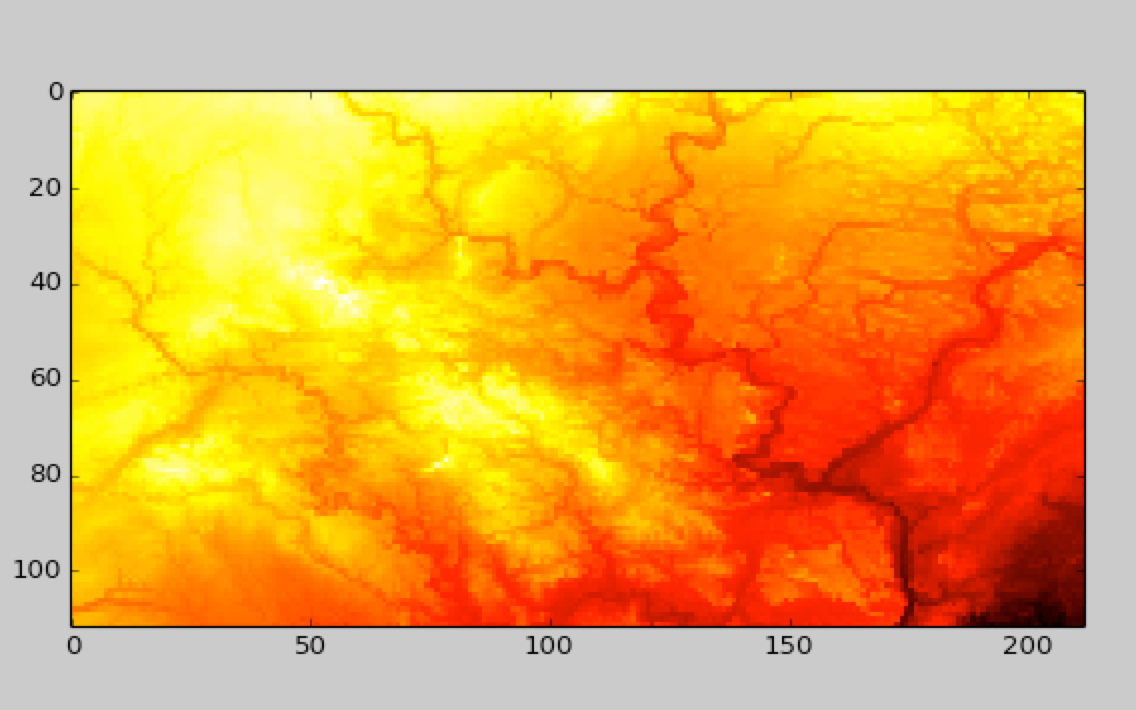
\includegraphics[width=0.4\textwidth]{images/heightmap_orig.png}}
\caption{200 by 100 heightmap of the Waterloo region}
\label{fig}
\end{figure}
where $1 unit * 6 \frac{arcsecond}{unit} * 30 \frac{meters}{arcsecond} = 180m$

In the reduction of the heightmap to a node graph, each unit square is represented by a waypoint. Thus this heightmap will reduce to a node graph with $200 * 100 = 20000$ nodes. In order to reduce the runtime of the proposed solution, reduce the complexity of the graph by only looking at the top left 20 by 10 section of the original heightmap. This is shown below
\begin{figure}[htbp] \label{img:heightmap2}
\centerline{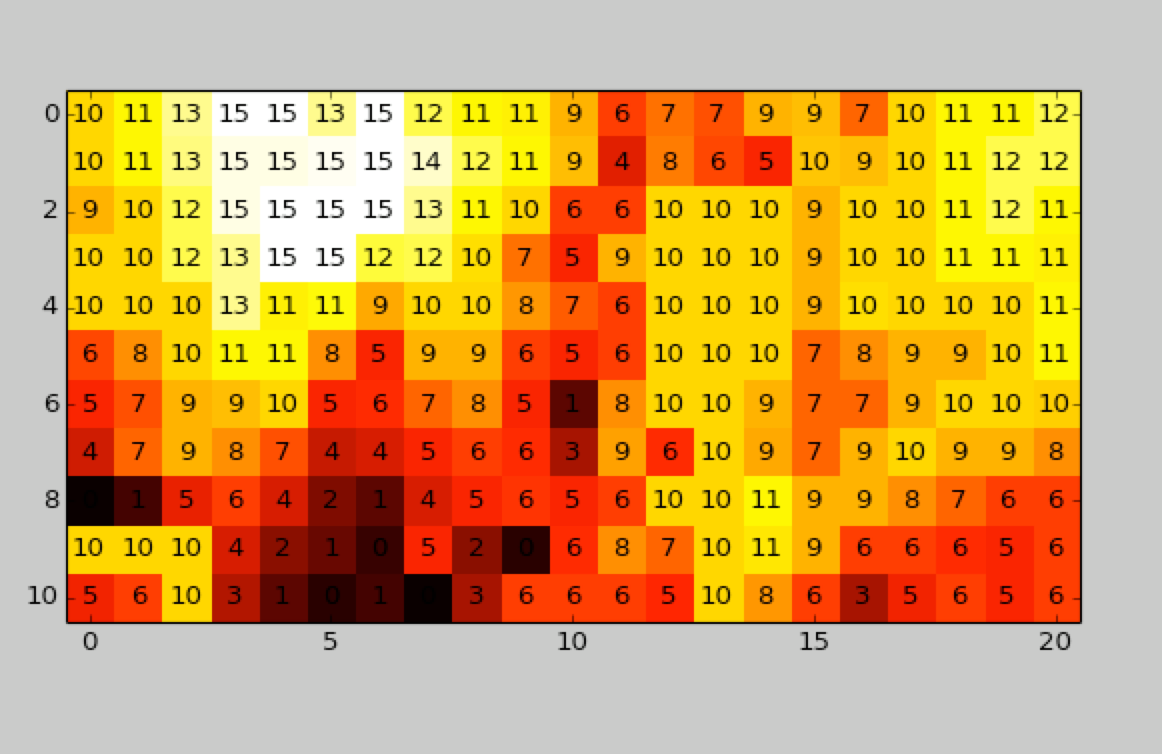
\includegraphics[width=0.4\textwidth]{images/heightmap.png}}
\caption{20 by 10 heightmap of the Waterloo region}
\label{fig}
\end{figure}
where the number at cell $(x, y)$ represents the value of $H(x, y)$.

Consider a 5 by 5 section of \ref{img:heightmap2} centered at $(x, y) = (10, 5)$, then the associate reduced node graph would look like
\begin{figure}[htbp] \label{img:nodegraph5}
\centerline{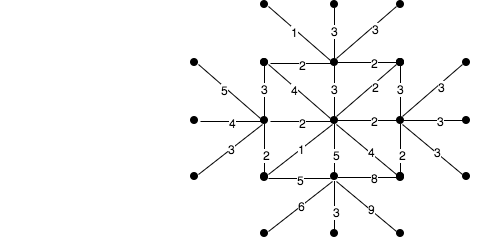
\includegraphics[width=0.4\textwidth]{images/nodegraph5.png}}
\caption{Reduced node graph for 5 by 5 of \ref{img:heightmap2}}
\label{fig}
\end{figure}

\subsection{Initial Solution}
Given lol, an initial solution $S$ is illustrated below
\begin{figure}[htbp] \label{img:solution_aco}
\centerline{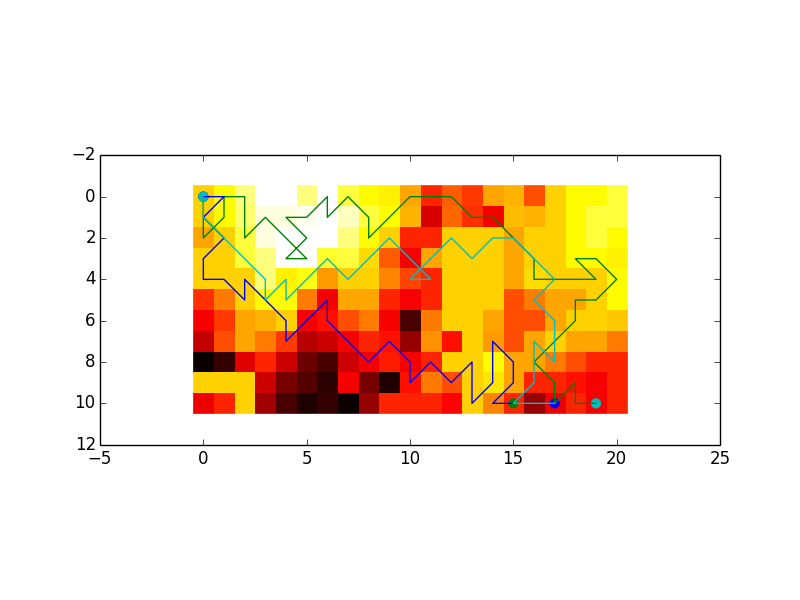
\includegraphics[width=0.4\textwidth]{images/solution_aco.png}}
\caption{Sample initial solution for problem}
\label{fig}
\end{figure}

\subsection{Solving Strategy}
Clearly, the initial solution is not optimal nor does it pass the goal test since it.

In order to optimize solution and evolve it towards the goal state, the paper proposes the use of ant colony optimization to optimize each of the drone's path from the start to end waypoints.

If ACO is used blindly for each drone, then there is no way to ensure that their paths won't collide. Therefore, a synchronization step is needed between all instances of the ACO algorithm to exchange information about the current path for each drone. To compute $C_{danger zones}(v_av_b)$ in \ref{eq:cost} for each drone, a priority order needs to be defined in order to deterministically state which danger zones are present in a certain drone's environment. Given $n$ drones with the ordering $d_1, ..., d_n$, then $d_i$ would contain the danger zones for all drones $1$ to $i-1$. Suppose the path for drone $i$ is $S_i$ where edge $v_av_b \in S_i$. Then $C_{danger zones}(v_av_b) = 10*n$ where $0 \leq n \leq i-1$ is the number of drones paths that contain the same edge $v_av_b$.

Finding the optimal ordering of $n$ drones that yields the lowest total path cost of all drones is a hard task. The proposed solution will use a permutation genetic algorithm to find this optimal ordering. The genotype of the algorithm is represented as an ordered list of drone IDs. This permutation genetic algorithm uses cycle-based crossover and the swap mutation operator. When selecting the members that survive to the next generation, the elitism model is used which keeps the fittest chromosome from each generation and replaces all other members.

\subsection{Cost Function}
Given a solution $S$ for $n$ drones, the cost for drone $i$ is 
\begin{equation} \label{eq:costdrone}
C_i = \sum_{j=1}^|S_i| C(S_i(j)) \quad \text{where} \quad C(v_av_b) \text{ is from \ref{eq:cost}}
\end{equation}

The cost of the entire solution $S$ is simply
\begin{equation} \label{eq:costsolution}
C_S = \sum_{i=1}^n C_i = \sum_{i=1}^n \sum_{j=1}^|S_i| C(S_i(j))
\end{equation}

\subsection{Neighbourhood Operator}
Within the context of the three-dimensional heightmap, the neighbourhood for a cell at $(x, y)$ contains all adjacent horizontal, vertical, and diagonal cells to $(x, y)$. Thus, when the heightmap is reduced to a node graph $G = (V, E)$, then $\forall v \in V$, $3 \leq deg(v) \leq 8$.

Assume the heightmap has width $w$ and length $l$. Let $f(v) : V \rightarrow [w, l] \times [w, l]$ return the cell location for a node in the original three-dimensional heightmap. Thus for drone $i$ with path $S_i$, the neighbourhood operate $N(v)$ is represented as
\begin{equation} \label{eq:neighbourhood}
N(v) = \{ u | abs(f(u) - f(v)) \leq (1, 1) \}
\end{equation}

% Talk about ACO ????
% Look at ant.py _pick_next:

\subsection{Parameter Selection}
\subsubsection{Genetic Algorithm}
For GA, the following parameters were used:\\
\textbf{Population size: } 200 \\
A large population size greatly increases the runtime of the GA algorithm, while a small population won't generate enough diversity to find a suitable path. A population size of 200 was the sweet spot that generated the most consistent solution under a good runtime.\\
\textbf{Iteration number: } 100 \\
Iteration number is similar to population size, as it increases runtime at large iterations, and decrease solution consistency at low iterations, an iteration number of 100 had consistent solution with good runtime \\
\textbf{Tournament size: } 10 \\
Tournament size affects the possibility that a non-optimal parent to be selected for cross over. The greater the tournament size, the less likely that will happen. A tournament size of 10 ensured that an optimal parent will be picked most of the time, and only occasionally a non-optimal parent is picked.\\
\textbf{Elitism rate: } 0.4 \\
Elitism rate affects the number of survivors for each generation. A rate of 0.4, in other words the top 40 percent of the parent will survive, ensures that most of the good solutions will be kept, and the algorithm will run in reasonable time since less children need to be computed to fill up the population.\\
\textbf{Mutation rate: } 0.4 \\
Mutation rate allows the algorithm to escape local minima. A mutation rate of 0.4 ensures that the entire search space will likely be searched, therefore improving the final solution of the algorithm.
\subsubsection{Ant Colony Optimization}
For ACO, the following parameters were used:\\
\textbf{Ant colony size: } 8 \\
A large ant colony size greatly increases the runtime of the ACO algorithm, while a small ant colony size won't generate enough diversity to find a suitable path. An ant colony size of 8 was the sweet spot that generated the most consistent solution under a good runtime.\\
\textbf{Iteration number: } 100 \\
Iteration number is similar to ant colony size, as it increases runtime at large iterations, and decrease solution consistency at low iterations, an iteration number of 100 had consistent solution with good runtime \\
\textbf{Alpha: } 0.5 \\
The alpha value affects the influence of pheromones on the ant's decision when choosing the next node to take. The greater the alpha value, the more likely an ant will choose a node based on the amount of pheromones already deposited. An alpha value of 0.5 ensured that choosing a path based on pheromones will be picked half of the time, giving emphasis to the cost of the path as well.\\
\textbf{Beta: } 1.2 \\
The beta value affects the influence of the path cost on the ant's decision when choosing the next node to take. The greater the beta value, the more likely an ant will choose a node based on its distance cost. A beta value of 1.2 ensured choosing a lower cost path. \\
\textbf{Evaporation rate: } 0.4 \\
Evaporation rate is how fast pheromones are evaporated from the edges of the graph. An evaporation rate of 0.4 ensures that the ants won't be bounded by old paths for a long period of time, which leads to new paths being discovered.

\subsection{Algorithm Demonstration}
\subsubsection{Genetic Algorithm}

\subsubsection{Ant Colony Optimization}

\subsection{Implementation}
The implementation for the proposed solution is located in the \verb|aco| directory. The file \verb|acosolver.py| in the root directory is the script used to run the proposed solution. The detailed instructions for usage of the script is in the user guide located in \verb|README| in the root project directory. 

\section{Performance Evaluation}
The metrics used for evaluating each meta-heuristic algorithm are runtime and the cost of the path taken. The experiments were ran using the height map of the region of Waterloo. This map contains 231 nodes and 830 edges. The experiments were conducted using varying numbers of drones. In each scenario, the parameters of GA and ACO are tuned to achieve the best performance. Ten trials were ran with each set of parameters and the averages of the results are listed below.

For a single drone, the results for ACO were the following:
\begin{center}
\begin{tabular}{ | m{1cm} | m{1cm}| m{1cm} | m{1.5cm} | m{1.5cm} |} 
\hline
number of ants & $\alpha$ & $\beta$ & path cost & runtime(s) \\ 
\hline
8 & 0.5 & 1.2 & 41.25 & 56.3 \\
\hline
16 & 0.5 & 1.2 & 37.25 & 97.1 \\ 
\hline
\end{tabular}
\end{center}

For a single drone, the results for GA were the following:
\begin{center}
\begin{tabular}{ | m{1.5cm} | m{1cm}| m{1cm} | m{1.5cm} | m{1.5cm} | m{1.5cm} |} 
\hline
tournament size & elitism rate & mutation rate & number of iterations & path cost & runtime(s) \\ 
\hline
10 & 0.2 & 0.7 & 100 & 40 & 58 \\ 
\hline
10 & 0.4 & 0.7 & 100 & 47.5 &  43  \\ 
\hline
30 & 0.2 & 0.7 & 100 & 47 &  57  \\ 
\hline
10 & 0.2 & 0.7 & 150 & 44.5 &  86  \\ 
\hline
\end{tabular}
\end{center}

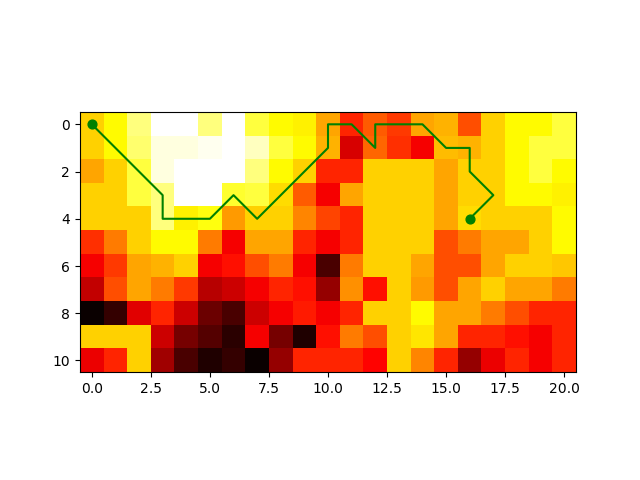
\includegraphics[scale=0.5]{performance/aco_1_drone}
Path generated using ACO

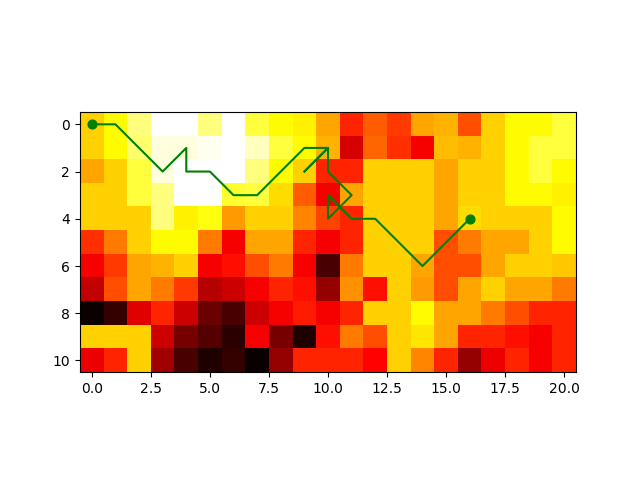
\includegraphics[scale=0.5]{performance/ga_1_drone}
Path generated using GA

Results for one drone: For GA, increasing the number of iterations, and varying the mutation rate and elitism rate and tournament size. The cost and time is worse than ACO

For two drones, the results for ACO were the following:
\begin{center}
\begin{tabular}{ | m{1cm} | m{1cm}| m{1cm} | m{1.5cm} | m{1.5cm} |} 
\hline
number of ants & $\alpha$ & $\beta$ & path cost & runtime(s) \\ 
\hline
8 & 0.5 & 1.2 & 53.75 & 83.5 \\ 
\hline
16 & 0.5 & 1.2 & 48.75 & 165.5 \\ 
\hline
\end{tabular}
\end{center}

For two drones, the results for GA were the following:
\begin{center}
\begin{tabular}{ | m{1.5cm} | m{1cm}| m{1cm} | m{1.5cm} | m{1.5cm} | m{1.5cm} |} 
\hline
tournament size & elitism rate & mutation rate & number of iterations & path cost & runtime(s) \\ 
\hline
10 & 0.2 & 0.7 & 100 & 53 & 112 \\ 
\hline
10 & 0.6 & 0.7 & 100 & 62 & 57  \\ 
\hline
30 & 0.2 & 0.7 & 100 & 59.25 & 112  \\ 
\hline
10 & 0.2 & 0.7 & 150 & 60 & 164  \\ 
\hline
\end{tabular}
\end{center}

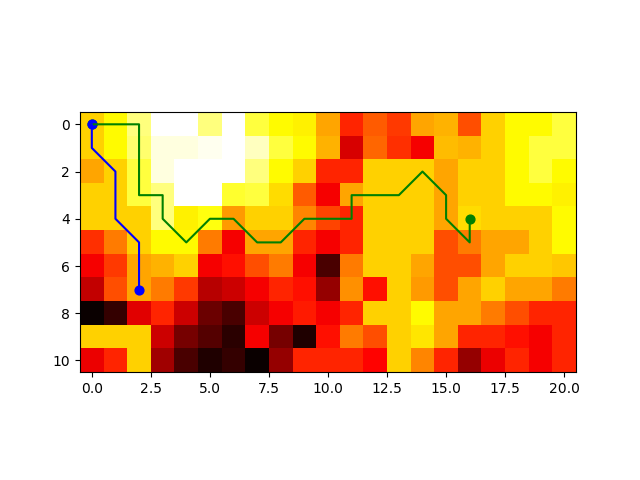
\includegraphics[scale=0.5]{performance/aco_2_drone}
Paths generated using ACO

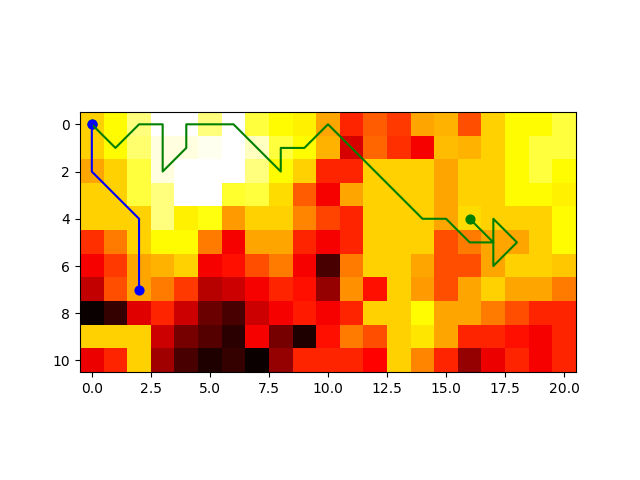
\includegraphics[scale=0.5]{performance/ga_2_drone}
Paths generated using GA

Results for two drones. Similar to the results for one drone, tuning the parameters of GA still results in worse cost compared to ACO. 

Based on the results between ACO and GA, it is clear that ACO has the better runtime performance. This shows that one of the advantages of ACO is that it uses parallelism which greatly improves the runtime of the algorithm. Speed is a big factor in drone delivery and so, a low runtime by ACO is preferred. In addition, by the graphs of the experiments, the paths produced by ACO seemed to be more optimal than the paths produced by GA. Unlike GA, ACO retains memory of the entire colony instead of just previous generation. This allows ACO to choose a better overall path. The disadvantage of ACO is that it uses a lot of parameters, and so the selection of values are mostly experimental. The alpha, beta, ant colony size and evaporation parameters were all determined through many rounds of trial and error until a decent path cost and runtime were observed. Furthermore, the number of iterations that was used in the experiments may not have achieved the best path. Increasing the number of iterations may take too long for a best solution to converge.

%TODO David talk about GA advantages/disadvantages

In addition, the usage of an A* algorithm for finding individual drone paths with GA running above it for determining an optimal ordering of the drones was conducted as a baseline. The heuristic function for each waypoint in the A* algorithm was based off the aforementioned cost function for mapping three-dimensional space into waypoints with the (x, y, z) positions being used to approximate distance to the goal. This baseline approach was found to perform worse than the above metaheuristic approaches with the following results:

With one drone:
\begin{center}
\begin{tabular}{ | m{1cm} | m{1cm}| m{1cm} | m{1.5cm} | m{1.5cm} |} 
\hline
path cost & runtime(s) \\ 
\hline
55.75 & 14.0 \\
\hline
\end{tabular}
\end{center}

With two drones:
\begin{center}
\begin{tabular}{ | m{1cm} | m{1cm}| m{1cm} | m{1.5cm} | m{1.5cm} |} 
\hline
path cost & runtime(s) \\ 
\hline
57.25 & 17.6 \\
\hline
\end{tabular}
\end{center}

Tests were also conducted with various other combinations of parameters for ACO which resulted in worse performance or worse results. The results for these tests are as follows:
\begin{center}
\begin{tabular}{ | m{1cm} | m{1cm}| m{1cm} | m{1.5cm} | m{1.5cm} |} 
\hline
number of drones & number of ants & $\alpha$ & $\beta$ & path cost & runtime(s) \\ 
\hline
1 & 8 & 0.3 & 0.9 & 48.25 & 72.4 \\
\hline
1 & 16 & 0.3 & 0.9 & 43.25 & 101.3 \\ 
\hline
1 & 8 & 1.2 & 0.5 & 46.5 & 55.8 \\
\hline
1 & 16 & 1.2 & 0.5 & 41.5 & 92.4 \\
\hline
2 & 8 & 0.3 & 0.9 & 59 & 90.6 \\
\hline
2 & 16 & 0.3 & 0.9 & 57.25 & 192.4 \\ 
\hline
2 & 8 & 1.2 & 0.5 & 57.5 & 86.4 \\
\hline
2 & 16 & 1.2 & 0.5 & 55 & 178.2 \\
\hline
\end{tabular}
\end{center}

\section{Conclusions \& Recommendations}
% TODO: Zuqi
For determining the optimal flight path of multiple package delivering drones for the Amazon Prime Air Traffic Control, a pure GA path finder algorithm and a combined ACO and GA path finder algorithm were implemented. Each algorithm will optimize the drones' flight paths given a region of height map, a set of initial locations, and a set of destinations. The fitness/cost function of both algorithms is defined as the sum of the distance cost, the height cost, and the danger zone cost. A danger zone is defined as the points of intersections between drones.

The pure GA algorithm optimizes the path of a single drone by performing the Simple GA algorithm. It uses one-point crossover, uniform mutation, and elitism survivor selection on an initial population of unoptimized drone paths for a pre-configured number of generations. The algorithm performs the Simple GA algorithm for each drone until each path is generated. On the other hand, the combined ACO and GA algorithm first uses a Permutation GA algorithm to determine the order of the drones' path to be calculated. It then uses the standard ACO algorithm to determine the path of each drone. Specifically, the solver's Permutation GA algorithm uses the cycle-based crossover, swap mutation, and elitism survivor selection to determine 10 drone orderings, and for each ordering, the algorithm performs ACO on each drone to generate its respective path. This entire process is repeated for a pre-configured number of generations until the optimal result is returned.

Both the pure GA and the combined ACO and GA algorithm solve the problem of coordinating multiple drones delivering packages to and from different destinations. This is solved by incorporating the distance, height, and previous drone paths into the fitness/cost functions of each algorithm in order to find the optimal result. Although both algorithms generates suitable paths for multiple drones, the results show that the combined ACO and GA algorithm performs slightly better than the pure GA algorithm overall in terms of the ratio between the path cost and runtime. However, the pure GA algorithm is slightly less consistent and sometimes outperforms the combined ACO and GA algorithm.

The combined ACO and GA algorithm is recommended based on the results shown in the performance evaluation. In addition, it optimizes the order of the drones while the pure GA algorithm generates the paths of the drones in a fixed order. Therefore, in theory, the combined ACO and GA algorithm is a superior program.

The proposed solution can be refined by incorporating a more complex cost function. The current implementation does not take into account of drone fuel, power, and ground collision. In addition, the danger zone cost of the current implementation can also be improved by incorporating time. Instead of increasing the cost of previous drones' entire paths, the algorithm can instead predict the position of the other drones at a given time in order to have a more realistic cost function. As a result, this should improve the overall path of the drones as well.

\begin{thebibliography}{00}
\bibitem{b1} Roberge, Vincent, Mohammed Tarbouchi, and Gilles Labont. ``Comparison of parallel genetic algorithm and particle swarm optimization for real-time UAV path planning.'' IEEE Transactions on Industrial Informatics 9.1 (2013): 132-141
\bibitem{b2} Tu, Jianping, and Simon X. Yang. ``Genetic algorithm based path planning for a mobile robot.'' Robotics and Automation, 2003. Proceedings. ICRA'03. IEEE International Conference on. Vol. 1. IEEE, 2003
\bibitem{b3} Masehian, Ellips, and DavoudSedighizadeh. ``A multi-objective PSO-based algorithm for robot path planning.'' Industrial Technology (ICIT), 2010 IEEE International Conference on. IEEE, 2010
\end{thebibliography}

\end{document}
